\documentclass[11pt,a4paper]{article}
%%%%%%%%%%%%%%%%%%%%%%%%% Credit %%%%%%%%%%%%%%%%%%%%%%%%

% template ini dibuat oleh martin.manullang@if.itera.ac.id untuk dipergunakan oleh seluruh sivitas akademik itera.

%%%%%%%%%%%%%%%%%%%%%%%%% PACKAGE starts HERE %%%%%%%%%%%%%%%%%%%%%%%%
\usepackage{graphicx}
\usepackage{caption}
\captionsetup[table]{name=Tabel}
\captionsetup[figure]{name=Gambar}
\usepackage{tabulary}
% \usepackage{amsmath}
\usepackage{fancyhdr}
% \usepackage{amssymb}
% \usepackage{amsthm}
\usepackage{placeins}
% \usepackage{amsfonts}
\usepackage{graphicx}
\usepackage[all]{xy}
\usepackage{tikz}
\usepackage{verbatim}
\usepackage[left=2cm,right=2cm,top=3cm,bottom=2.5cm]{geometry}
\usepackage{hyperref}
\hypersetup{
    colorlinks,
    linkcolor={red!50!black},
    citecolor={blue!50!black},
    urlcolor={blue!80!black}
}
\usepackage{libertine}
\usepackage{libertinust1math}
\usepackage[T1]{fontenc}
\usepackage{inconsolata}

\usepackage{caption}
\usepackage{subcaption}
\usepackage{multirow}
\usepackage{psfrag}
\usepackage[T1]{fontenc}
\usepackage[scaled]{beramono}
% Enable inserting code into the document
\usepackage{listings}
\usepackage{xcolor} 
% custom color & style for listing
\definecolor{codegreen}{rgb}{0,0.6,0}
\definecolor{codegray}{rgb}{0.5,0.5,0.5}
\definecolor{codepurple}{rgb}{0.58,0,0.82}
\definecolor{backcolour}{rgb}{0.95,0.95,0.92}
\lstdefinestyle{mystyle}{
	backgroundcolor=\color{backcolour},   
	commentstyle=\color{green},
	keywordstyle=\color{codegreen},
	numberstyle=\tiny\color{codegray},
	stringstyle=\color{codepurple},
	basicstyle=\ttfamily\footnotesize,
	breakatwhitespace=false,         
	breaklines=true,                 
	captionpos=b,                    
	keepspaces=true,                 
	numbers=left,                    
	numbersep=5pt,                  
	showspaces=false,                
	showstringspaces=false,
	showtabs=false,                  
	tabsize=2
}
\lstset{style=mystyle}
\renewcommand{\lstlistingname}{Kode}
%%%%%%%%%%%%%%%%%%%%%%%%% PACKAGE ends HERE %%%%%%%%%%%%%%%%%%%%%%%%


%%%%%%%%%%%%%%%%%%%%%%%%% Data Diri %%%%%%%%%%%%%%%%%%%%%%%%
\newcommand{\stuid}{120140154}
\newcommand{\student}{\textbf{Ryan Ernanda (\stuid{})}}
\newcommand{\course}{\textbf{Sistem Operasi-RB (IF2223)}}
\newcommand{\assignment}{\textbf{2}} % tugas ke...

%%%%%%%%%%%%%%%%%%% using theorem style %%%%%%%%%%%%%%%%%%%%
\newtheorem{thm}{Theorem}
\newtheorem{lem}[thm]{Lemma}
\newtheorem{defn}[thm]{Definition}
\newtheorem{exa}[thm]{Example}
\newtheorem{rem}[thm]{Remark}
\newtheorem{coro}[thm]{Corollary}
\newtheorem{quest}{Question}[section]
%%%%%%%%%%%%%%%%%%%%%%%%%%%%%%%%%%%%%%%%
\usepackage{lipsum}%% a garbage package you don't need except to create examples.
\usepackage{fancyhdr}
\usepackage[ddmmyyyy]{datetime}
\pagestyle{fancy}
\lhead{Ryan Ernanda (120140154)}
\rhead{ \thepage}
\cfoot{\textbf{HandsOn 2 : Synchronisation and Deadlock}} % ini untuk judul tugas
\renewcommand{\headrulewidth}{0.4pt}
\renewcommand{\footrulewidth}{0.4pt}

%%%%%%%%%%%%%%  Shortcut for usual set of numbers  %%%%%%%%%%%

\newcommand{\N}{\mathbb{N}}
\newcommand{\Z}{\mathbb{Z}}
\newcommand{\Q}{\mathbb{Q}}
\newcommand{\R}{\mathbb{R}}
\newcommand{\C}{\mathbb{C}}
\setlength\headheight{14pt}

%%%%%%%%%%%%%%%%%%%%%%%%%%%%%%%%%%%%%%%%%%%%%%%%%%%%%%%555

\begin{document}
\thispagestyle{empty}
\begin{center}
	
\includegraphics[scale = 0.15]{Figure/ifitera-header.png}
	\vspace{0.1cm}
\end{center}
\noindent
% change font family for header section only
%{\fontfamily{LinuxLibertineT-OsF}\large\selectfont 
{\large
\rule{17cm}{0.2cm}\\[0.3cm]
Nama: \student \hfill Tugas Ke: \assignment\\[0.1cm]
Mata Kuliah: \course \hfill Tanggal: 03/11/2022\\
\rule{17cm}{0.05cm}
\vspace{0.1cm}
}


%%%%%%%%%%%%%%%%%%%%%%%%%%%%%%%%%%%%%%%%%%%%% BODY DOCUMENT %%%%%%%%%%%%%%%%%%%%%%%%%%%%%%%%%%%%%%%%%%%%%
\section{Tujuan Hands On}
Dalam pengerjaan Handson 2 ini memiliki tujuan, yaitu:
\begin{itemize}
	\item Memahami sistem sinkronisasi dan permasalahan yang ada
	\item Memahami solusi dalam menangani \textit{critical section}
	\item Memahami implementasi dari :
		\begin{itemize}
			\item \textit{Join} mengunakan \textit{semaphores}
			\item \textit{Binary semaphores}
			\item \textit{Producer Consumer}
			\item \textit{Reader / Writer}
			\item \textit{Dining Philosophers}
		\end{itemize}
\end{itemize}

\section{Spesifikasi Sistem}
    Perangkat lunak yang saya gunakan sebagai virtual dari sistem operasi adalah \textit{Oracle VM VirtualBox} versi 6.1, dan spesifikasi dari sistem operasi linux Ubuntu yaitu 2 GB RAM, 13 GB \textit{storage}, 16 MB VRAM, 1 CPU \textit{Processors}. 
    \begin{figure}[h]
    \centering
    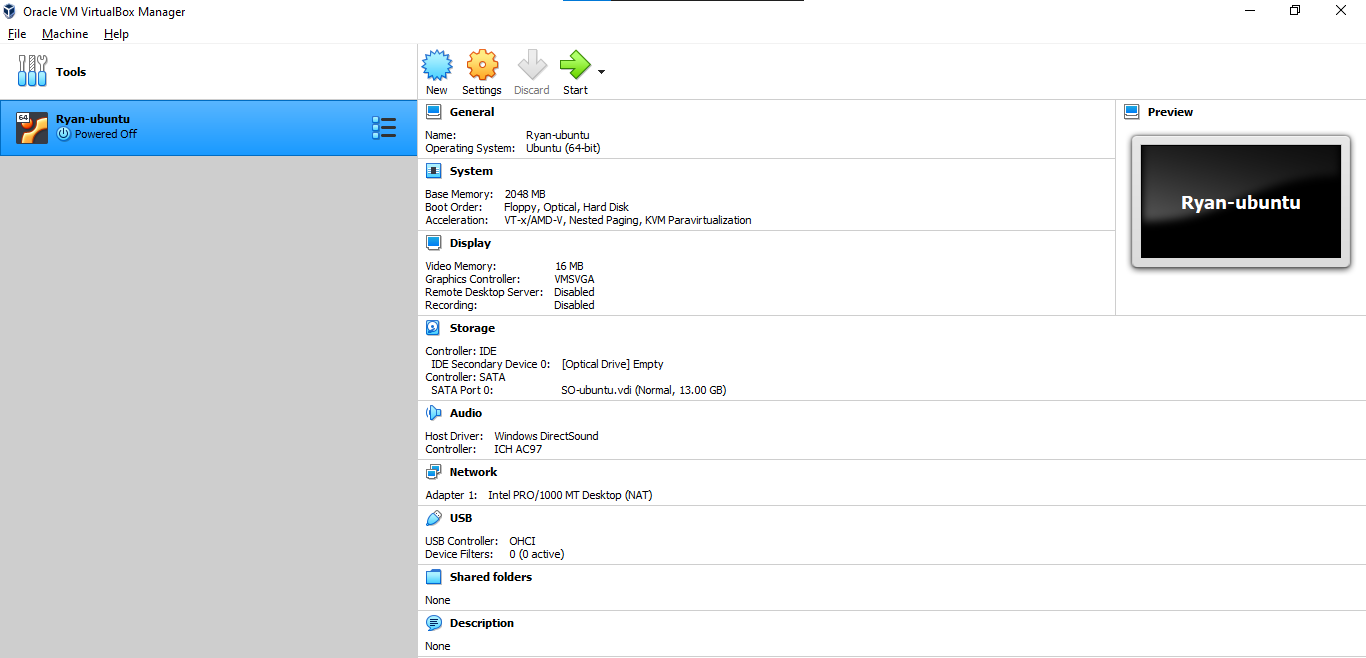
\includegraphics[width=0.8\textwidth]{Figure/Spek.png}
    \caption{Spesifikasi Sistem Operasi}
    \label{fig:my_label}
    \end{figure}

\section{\textit{Fork / Join}}
\subsection{\textit{Source Code}}
\begin{lstlisting}[language=C]
	sem_t s;

	void *child(void *arg) {
		sleep(2);
		printf("child\n");
		Sem_post(&s); // signal here: child is done
		return NULL;
	}

	int main(int argc, char *argv[]) {
		Sem_init(&s, 0); 
		printf("parent: begin\n");
		pthread_t c;
		Pthread_create(&c, NULL, child, NULL);
		Sem_wait(&s); // wait here for child
		printf("parent: end\n");
		return 0;
	}
	
\end{lstlisting}

\subsection{\textit{Output}}
\begin{figure}[h]
    \centering
    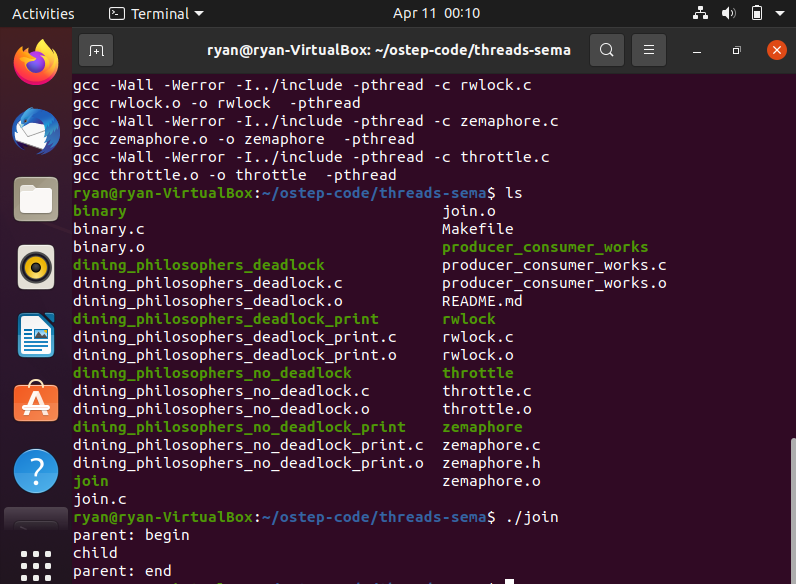
\includegraphics[width=0.8\textwidth]{Figure/Frok join.png}
    \caption{Fork/Join}
    \label{fig:my_label}
\end{figure}

    
\subsection{Penjelasan}
     \textit{Semaphore} adalah struktur data komputer yang berguna untuk sinkronisasi proses serta berfungsi dalam  kontrol program untuk mengeksekusi proses. Contohnya yaitu pada suatu \textit{thread} yang sedang menunggu \textit{list} agar \textit{list} itu tidak dalam keadaan kosong. Kondisi ini diartikan \textit{sem init} menjadi '0'. Jika pembuatan \textit{threads} tersebut sudah selesai maka akan diteruskan ke pemanggilan \textit{child semaphore} yang memberi sinyal karena proses \textit{child} sudah selesai dan melakukan \textit{return}. Jika \textit{child} selesai, maka \textit{semaphore} melanjukan prosesnya dan melakukan \textit{output 'parent : end'}. Dalam implementasinya terdapat fungsi \textit{Sem wait & Sem post} yang digunakan untuk menunggu \textit{child} dari \textit{parent} selesai. kode tersebut menunjukkan bahwa nilai semaphore harus diubah menjadi 0, jika kondisi ini tidak terpenuhi, \textit{parent} terlebih dahulu akan  memanggil fungsi \textit{sem wait} sebelum \textit{child} selesai memanggil fungsi \textit{sem post}. hal ini dapat dilihat bahwa nilai \textit{semaphore} lebih besar dari 0 maka akan membuatnya tertidur selama 2 detik. Jika nilai \textit{semaphore} sama dengan 0,  program memulai eksekusi dari \textit{parent} dan berakhir.

\section{\textit{Binary Semaphores}}
\subsection{\textit{Source Code}}
    \begin{lstlisting}[language = C]
	volatile int counter = 0;

	void *child(void *arg) {
		int i;
		for (i = 0; i < 10000000; i++) {
		Sem_wait(&mutex);
		counter++;
		Sem_post(&mutex);
		}
		return NULL;
	}

	int main(int argc, char *argv[]) {
		Sem_init(&mutex, 1); 
		pthread_t c1, c2;
		Pthread_create(&c1, NULL, child, NULL);
		Pthread_create(&c2, NULL, child, NULL);
		Pthread_join(c1, NULL);
		Pthread_join(c2, NULL);
		printf("result: %d (should be 20000000)\n", counter);
		return 0;
	}
\end{lstlisting}
    \subsection{\textit{Output}}
    \begin{figure}[h]
    \centering
    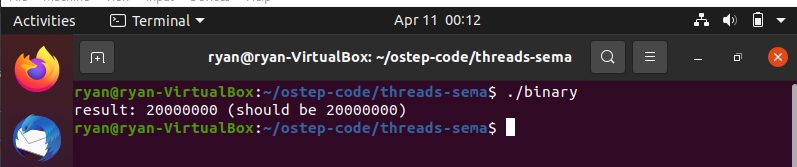
\includegraphics[width=1\textwidth]{Figure/Binary.png}
    \caption{Binary Semaphores}
    \label{fig:my_label}
    \end{figure}

\subsection{Penjelasan}
    Penggalan kode tersebut memiliki variabel \textit{mutual exclusion} atau dikenal dengan \textit{sem t mutex} yang memiliki fungsi dalam mengontrol \textit{resource} dan mencegah adanya kondisi \textit{race}. Pertama \textit{mutex} tersebut di inisialisasikan dengan \textit{value} yaitu 1 yang selanjutnya dibuat \textit{thread} yang memiliki inisial c1 dan c2, c1 dan c2 ini berguna dalam menjalankan \textit{child}, kemudian ada inisialisasi i guna untuk melakukan perulangan \textit{for} hingga nilai i kurang dari 10000000, dan perulangan ini menjalankan \textit{sem wait} yang valuenya juga akan berkurang hingga terjadi \textit{critical section}. Untuk nilai \textit{counter} akan ada penambahan dimana \textit{semaphore} melakukan proses \textit{calling} dengan cara menambah \textit{value} dari \textit{semaphore} tersebut yang dimana proses ini merupakan tanda dari \textit{critical section} yang sudah selesai. Selanjutnya, pengulangan terus terjadi hingga syarat terpenuhi dan akan dilanjutkan oleh \textit{thread} c2 untuk melakukan fungsi \textit{child}, jika sudah selesai, maka selanjutnya me-\textit{return} ke fungsi \textit{main} dan keluar output yang telah dijalankan dari menampilkan hasil counter, output ini bernilai 20000000.
 
\section{\textit{Producer Consumer}}
\subsection{\textit{Source Code}}
\begin{lstlisting}[language = C]
	int max;
	int loops;
	int *buffer;

	int use  = 0;
	int fill = 0;

	sem_t empty;
	sem_t full;
	sem_t mutex;

	#define CMAX (10)
	int consumers = 1;

	void do_fill(int value) {
		buffer[fill] = value;
		fill++;
		if (fill == max)
		fill = 0;
	}

	int do_get() {
		int tmp = buffer[use];
		use++;
		if (use == max)
		use = 0;
		return tmp;
	}

	void *producer(void *arg) {
		int i;
		for (i = 0; i < loops; i++) {
		Sem_wait(&empty);
		Sem_wait(&mutex);
		do_fill(i);
		Sem_post(&mutex);
		Sem_post(&full);
		}

		// end case
		for (i = 0; i < consumers; i++) {
		Sem_wait(&empty);
		Sem_wait(&mutex);
		do_fill(-1);
		Sem_post(&mutex);
		Sem_post(&full);
		}

		return NULL;
	}
																				
	void *consumer(void *arg) {
		int tmp = 0;
		while (tmp != -1) {
		Sem_wait(&full);
		Sem_wait(&mutex);
		tmp = do_get();
		Sem_post(&mutex);
		Sem_post(&empty);
		printf("%lld %d\n", (long long int) arg, tmp);
		}
		return NULL;
	}

	int main(int argc, char *argv[]) {
		if (argc != 4) {
		fprintf(stderr, "usage: %s <buffersize> <loops> <consumers>\n", argv[0]);
		exit(1);
		}
		max   = atoi(argv[1]);
		loops = atoi(argv[2]);
		consumers = atoi(argv[3]);
		assert(consumers <= CMAX);

		buffer = (int *) malloc(max * sizeof(int));
		assert(buffer != NULL);
		int i;
		for (i = 0; i < max; i++) {
		buffer[i] = 0;
		}

		Sem_init(&empty, max); // max are empty 
		Sem_init(&full, 0);    // 0 are full
		Sem_init(&mutex, 1);   // mutex

		pthread_t pid, cid[CMAX];
		Pthread_create(&pid, NULL, producer, NULL); 
		for (i = 0; i < consumers; i++) {
		Pthread_create(&cid[i], NULL, consumer, (void *) (long long int) i); 
		}
		Pthread_join(pid, NULL); 
		for (i = 0; i < consumers; i++) {
		Pthread_join(cid[i], NULL); 
		}
		return 0;
	}
\end{lstlisting}
\newpage
   \subsection{\textit{Output}}
    \begin{figure}[h]
	\centering
	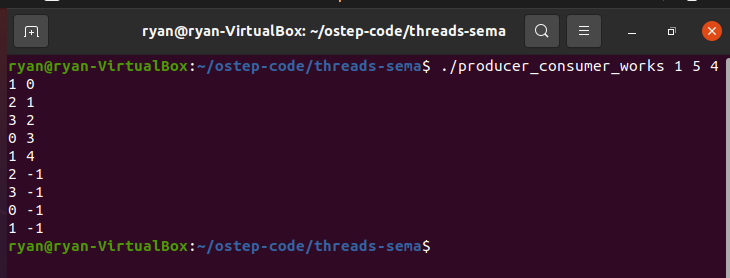
\includegraphics[width=0.8\textwidth]{Figure/producer_consumer_works.png}
	\caption{Produce Consumer}
    \end{figure}
    
\subsection{Penjelasan}
    Dalam implementasi ini kita dapat menyebutnya sebagai \textit{bounded buffer}. Program menjalankan fungsi prosedural yang berguna untuk memanggil\textit{sem wait (empty)} dan \textit{sem post (mutex)}. Prosedur ini berlanjut hingga yang \textit{empty} menjadi nilai \textit{max}. \textit{Producer} akan mengisi fungsi \textit{do fill} dengan entri \textit{buffer} pertama  setelah \textit{empty} berkurang hingga mencapai nilai 0. Kemudian Producer akan terus berjalan sampai suatu saat  memanggil \textit{Sem post(mutex)} dan \textit{Sem post(full)}  akan merubah nilai  full dari  -1 menjadi 0. Maka \textit{Consumer} akan melakukan perulangan dan block dengan nilai semaphore yang kosong. Jika terjadi kondisi di mana \textit{producer} terganggu, fungsi \textit{consumer} mulai melakukan pengembalian dari batas  \textit{sem wait(full)}, dan kemudian menggunakan \textit{buffer} eksekusi fungsi \textit{do get}. Keadaan kedua \textit{producer} akan terganggu jika keduanya menjalankan fungsi \textit{do fill} secara bersamaan. Kondisi \textit{interruped} juga terjadi jika \texitf{producer} 1 mengisi \textit{entry buffer} untuk pertama kalinya, sedangkan ketika kesempatan mengisinya belum selesai, \textit{producer} 1 akan \textit{interruped}. Pada titik ini, \textit{producer} 2 mengimplementasikan fungsi \texit{buffer} karena menyisipkan elemen ke dalam \texit{buffer}, yang berarti bahwa data lama akan ditimpa olehnya. Oleh karena itu,  \texit{semaphore binary} diperlukan, dan \texit{locks} ditambahkan untuk menghindari \texit{deadlock}. dari itu \texit{consumer} mengambil langkah pertama dengan memanggil \texit{Sem wait(full)} karena data belum tersedia. Dengan panggilan ini \texit{consumer} akan memblokir, kemudian produser akan berjalan, yang memulai \texit{consumer thread} dan panggilan \texit{sem wait(mutex} dengan \texit{producer} diblokir atau terhenti.


\section{\textit{Reader / Writer}}
    \subsection{\textit{Source Code}}
    \begin{lstlisting}[language = C]		
	int read_loops;
	int write_loops;
	int counter = 0;

	rwlock_t mutex;

	void *reader(void *arg) {
		int i;
		int local = 0;
		for (i = 0; i < read_loops; i++) {
		rwlock_acquire_readlock(&mutex);
		local = counter;
		rwlock_release_readlock(&mutex);
		printf("read %d\n", local);
		}
		printf("read done: %d\n", local);
		return NULL;
	}

	void *writer(void *arg) {
		int i;
		for (i = 0; i < write_loops; i++) {
		rwlock_acquire_writelock(&mutex);
		counter++;
		rwlock_release_writelock(&mutex);
		}
		printf("write done\n");
		return NULL;
	}

	int main(int argc, char *argv[]) {
		if (argc != 3) {
		fprintf(stderr, "usage: rwlock readloops writeloops\n");
		exit(1);
		}
		read_loops = atoi(argv[1]);
		write_loops = atoi(argv[2]);
		
		rwlock_init(&mutex); 
		pthread_t c1, c2;
		Pthread_create(&c1, NULL, reader, NULL);
		Pthread_create(&c2, NULL, writer, NULL);
		Pthread_join(c1, NULL);
		Pthread_join(c2, NULL);
		printf("all done\n");
		return 0;
	}
\end{lstlisting}
  \subsection{\textit{Output}}
    \begin{figure}[h]
	\centering
	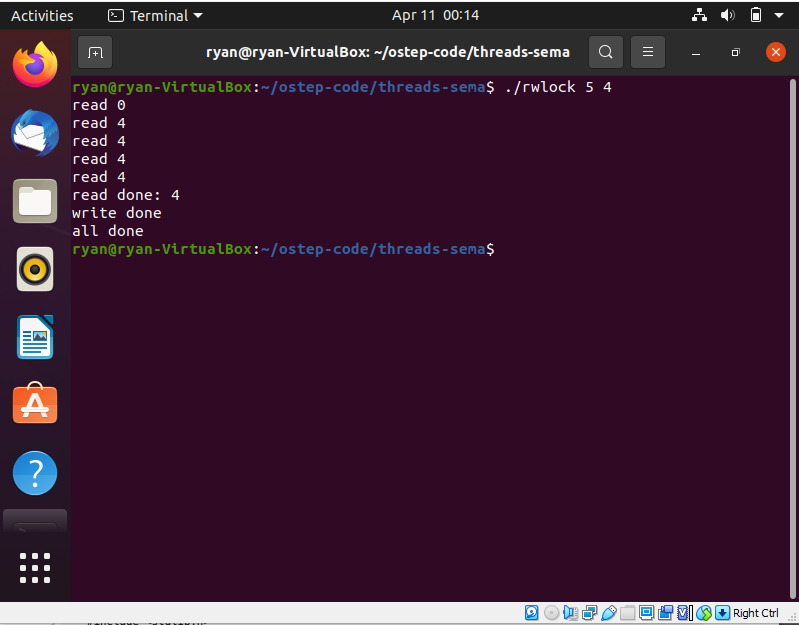
\includegraphics[width=0.6\textwidth]{Figure/rwlocks.png}
	\caption{Reader / Writer}
    \end{figure}
    \subsection{Penjelasan}
    Program diatas merupakan implementasi \texit{Reader / Writer Locks}. Jika \texit{thread} suatu saat memperbarui strukturnya agar bisa melakukan panggilan pasangan operasi sinkron \texit{rwlock acquire writelock} dimana ini memiliki fungsi untuk melepaskan \texit{writelock & rwlock release}. Semaphore \texit{writelock} ini memastikan hanya satu \texit{writer} yang dapat di \texit{lock} dan memperbarui struktur datanya dengan cara memasuki \texit{critical section}. Ketika \texit{lock} didapati maka \texit{reader} pertama akan mendapatkan \texit{lock} tersebut serta menambahkan variabel \texit{reader} supaya bisa melacak beberapa \texit{reader} pada struktur data ini. Jika semua \texit{threads} terdapat \texit{writelock} maka wajib bagi \texit{threads} ini untuk menunggu hingga semua \texit{reader} telah selesai. 

\section{\textit{Dining Philosophers}}
\subsection{\textit{Dining Philosophers Deadlock}}
\subsubsection{\textit{Source Code}}
\begin{lstlisting}[language = C]

	void space(int s) {
		Sem_wait(&print_lock);
		int i;
		for (i = 0; i < s * 10; i++)
		printf(" ");
	}
	
	void space_end() {
		Sem_post(&print_lock);
	}
	
	int left(int p)  {
		return p;
	}
	
	int right(int p) {
		return (p + 1) % 5;
	}
	
	void get_forks(int p) {
		space(p); printf("%d: try %d\n", p, left(p)); space_end();
		Sem_wait(&forks[left(p)]);
		space(p); printf("%d: try %d\n", p, right(p)); space_end();
		Sem_wait(&forks[right(p)]);
	}
	
	void put_forks(int p) {
		Sem_post(&forks[left(p)]);
		Sem_post(&forks[right(p)]);
	}
	
	void think() {
		return;
	}
	
	void eat() {
		return;
	}
	
	void *philosopher(void *arg) {
		arg_t *args = (arg_t *) arg;
	
		space(args->thread_id); printf("%d: start\n", args->thread_id); space_end();
	
		int i;
		for (i = 0; i < args->num_loops; i++) {
		space(args->thread_id); printf("%d: think\n", args->thread_id); space_end();
		think();
		get_forks(args->thread_id);
		space(args->thread_id); printf("%d: eat\n", args->thread_id); space_end();
		eat();
		put_forks(args->thread_id);
		space(args->thread_id); printf("%d: done\n", args->thread_id); space_end();
		}
		return NULL;
	}
																				 
	int main(int argc, char *argv[]) {
		if (argc != 2) {
		fprintf(stderr, "usage: dining_philosophers <num_loops>\n");
		exit(1);
		}
		printf("dining: started\n");
		
		int i;
		for (i = 0; i < 5; i++) 
		Sem_init(&forks[i], 1);
		Sem_init(&print_lock, 1);
	
		pthread_t p[5];
		arg_t a[5];
		for (i = 0; i < 5; i++) {
		a[i].num_loops = atoi(argv[1]);
		a[i].thread_id = i;
		Pthread_create(&p[i], NULL, philosopher, &a[i]);
		}
	
		for (i = 0; i < 5; i++) 
		Pthread_join(p[i], NULL); 
	
		printf("dining: finished\n");
		return 0;
	}
\end{lstlisting}

\subsubsection{\textit{Output}}
   \begin{figure}[h]
	\centering
	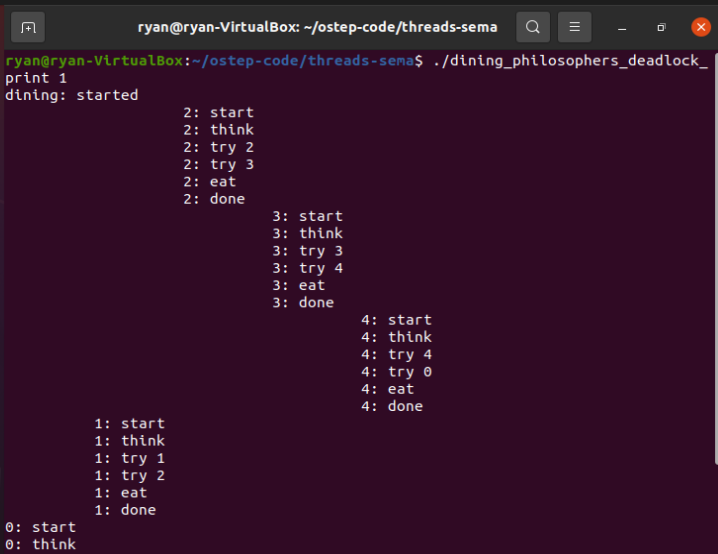
\includegraphics[width=0.8\textwidth]{Figure/dining_deadlock_print(1).png}
    \end{figure}
       \begin{figure}[h]
	\centering
	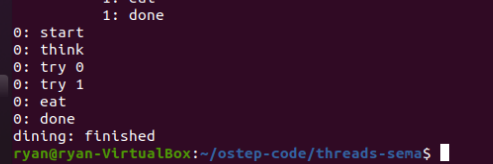
\includegraphics[width=0.8\textwidth]{Figure/dining_deadlock_print(2).png}
	\caption{Dining Philosophers Deadlock}
    \end{figure}

\subsubsection{Penjelasan}
 Ketika kondisi \texit{philosopher P} dirujuk ke \texit{fork} kiri maka akan mulai memanggil fungsi \texit{left}, dan sebaliknya. Terdapat \texit{modulo} dimana  \texit{modulo} ini menangani satu persoalan \texit{philosopher} akhir yang mana \texit{P=4} dan \texit{P} mengambil \texit{fork} bagian kanan ketika \texit{fork} bernilai kosong 
 
\subsection{\textit{Dining Philosophers No Deadlock}}
\subsubsection{\textit{Source Code}}
\begin{lstlisting}[language = C]
	void space(int s) {
		Sem_wait(&print_lock);
		int i;
		for (i = 0; i < s * 10; i++)
		printf(" ");
	}
	
	void space_end() {
		Sem_post(&print_lock);
	}
	
	int left(int p)  {
		return p;
	}
	
	int right(int p) {
		return (p + 1) % 5;
	}
	
	void get_forks(int p) {
		if (p == 4) {
		space(p); printf("4 try %d\n", right(p)); space_end();
		Sem_wait(&forks[right(p)]);
		space(p); printf("4 try %d\n", left(p)); space_end();
		Sem_wait(&forks[left(p)]);
		} else {
		space(p); printf("try %d\n", left(p)); space_end();
		Sem_wait(&forks[left(p)]);
		space(p); printf("try %d\n", right(p)); space_end();
		Sem_wait(&forks[right(p)]);
		}
	}
	
	void put_forks(int p) {
		Sem_post(&forks[left(p)]);
		Sem_post(&forks[right(p)]);
	}
	
	void think() {
		return;
	}
	
	void eat() {
		return;
	}
	
	void *philosopher(void *arg) {
		arg_t *args = (arg_t *) arg;
	
		space(args->thread_id); printf("%d: start\n", args->thread_id); space_end();
	
		int i;
		for (i = 0; i < args->num_loops; i++) {
		space(args->thread_id); printf("%d: think\n", args->thread_id); space_end();
		think();
		get_forks(args->thread_id);
		space(args->thread_id); printf("%d: eat\n", args->thread_id); space_end();
		eat();
		put_forks(args->thread_id);
		space(args->thread_id); printf("%d: done\n", args->thread_id); space_end();
		}
		return NULL;
	}
																				 
	int main(int argc, char *argv[]) {
		if (argc != 2) {
		fprintf(stderr, "usage: dining_philosophers <num_loops>\n");
		exit(1);
		}
		printf("dining: started\n");
		
		int i;
		for (i = 0; i < 5; i++) 
		Sem_init(&forks[i], 1);
		Sem_init(&print_lock, 1);
	
		pthread_t p[5];
		arg_t a[5];
		for (i = 0; i < 5; i++) {
		a[i].num_loops = atoi(argv[1]);
		a[i].thread_id = i;
		Pthread_create(&p[i], NULL, philosopher, &a[i]);
		}
	
		for (i = 0; i < 5; i++) 
		Pthread_join(p[i], NULL); 
	
		printf("dining: finished\n");
		return 0;
	}	
\end{lstlisting}
\subsubsection{\textit{Output}}
 \begin{figure}[h]
	\centering
	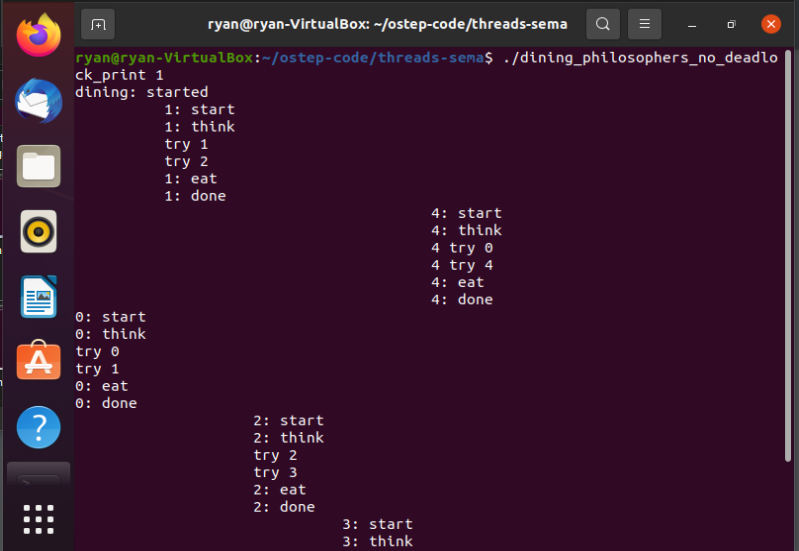
\includegraphics[width=0.6\textwidth]{Figure/dining_no_deadlock_print(1).png}
    \end{figure}
    \begin{figure}[h]
	\centering
	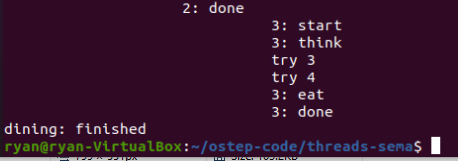
\includegraphics[width=0.8\textwidth]{Figure/dining_no_deadlock_print(2).png}
	\caption{Dining Philosophers No Deadlock}
    \end{figure}
\subsubsection{Penjelasan}
Kita perlu tahu bahwa \texit{philosophers} memiliki angka dan kita juga dapat menulis \texit{get forks} dan \texit{put forks} terus menerus. Setelah itu, kita perlu \texit{locks} untuk menemukan \texit{forks} dengan mengambil \texit{forks} kiri dan melanjutkan ke kanan. ketika selesai, itu pasti akan dilepas, tetapi kondisinya tidak terjadi karena \texit{deadlock}.
 
\section{Kesimpulan}
     Yang dapat saya simpulkan dalam menyelesaikan tugas HandsOn 2 ini yaitu saya belajar dan memahami tentang \texit{Synchronisation and Deadlock}. Tidak hanya itu saja, saya juga mengerti tentang penggunaan \texit{Semaphore} pada program yang telah diberikan \texit{programmer} tersebut.
     
\section{Link Google Drive}
Link Folder Assigment HandsOn 2 : \href{https://drive.google.com/drive/folders/1HrX1BeNBsXnGzcpViksC96O-c1VZsPWD?usp=sharing}{Klik Disini}.

\end{document}